\section{RANS wall-function fundamentals}
\label{sec:background:rans-wall-function-fundamentals}

This section is a brief intro to the idea of wall-functions and the difference from the universality of the boundary layers between incompressible and compressible turbulent boundary layers. For more details the reader is encourage to read Chapter 8 - "Wall Functions" of Hanjalic and Launder's "Modelling Turbulence in Engineering and the Environment" \cite{hanjalic2022modelling} - this section is far from a complete introduction.

\subsection{Spalding's law of the wall}
\label{subsec:background:spalding}
% Writing prerequisite for Chapter 7: give the unified viscous/logarithmic law,
% its near-wall limit and the roles of kappa and the log-law intercept.

Wall functions exploit \textit{some} approximate universality of the mean velocity profile in the inner region of smooth-wall turbulent flows. The dimensionless velocity and wall-normal distance are defined as \(u^+=u/u_\tau\) and \(y^+=yu_\tau/\nu\), respectively, where \(u\) is the mean tangential velocity, \(y\) is the distance from the wall, \(\nu\) is the kinematic viscosity, and \(u_\tau=\sqrt{\tau_w/\rho}\) is the friction velocity based on the wall shear stress \(\tau_w\) and fluid density \(\rho\). For incompressible, constant-property flows under approximately equilibrium conditions, profiles expressed in these wall units follow the linear relation \(u^+=y^+\) in the viscous sublayer and a logarithmic relation in the logarithmic region (see Figure~\ref{fig:background:spaldin_law-of-the-wall}). Spalding \cite{spalding1961single} combined these limiting behaviours into a single analytical interpolation spanning the viscous sublayer, blending in the buffer layer, and logarithmic region - often referred to as the universal or Spalding's law-of-the-wall. This lack of a universal law in the buffer layer is linked to general caution of using wall-functions in this specific region of \(5 \le y^+ \le 30\). Figure~\ref{fig:background:spaldin_law-of-the-wall} illustrates this blending and compares it with DNS and the two laws relations in the sublayer and log-layer respectively. Beyond the logarithmic region of the inner region of the boundary layer is the wake region, for which again special laws, such as Cole's law-of-the-wake \cite{coles1956law}. 

Such relations provide a basis for wall functions, which infer the wall shear stress from the resolved near-wall velocity and its distance from the wall, reducing the need to resolve the steep near-wall gradients explicitly. Figure~\ref{fig:background:wf-mesh} contrasts a wall-resolved mesh with a conventional wall-function mesh whose first cell centre lies in the logarithmic region. This reduction in near-wall mesh requirement reduces the computational time by reducing the overall cell number and the stiffness of the equation by avoiding the typically thin slivered cells directly at the wall \cite{ecca2015pros}. A formulation spanning all three regions is referred to as adaptive wall-function, and permits the first cell point to lie in different parts of the inner layer. 

\begin{figure}[H]
    \centering
    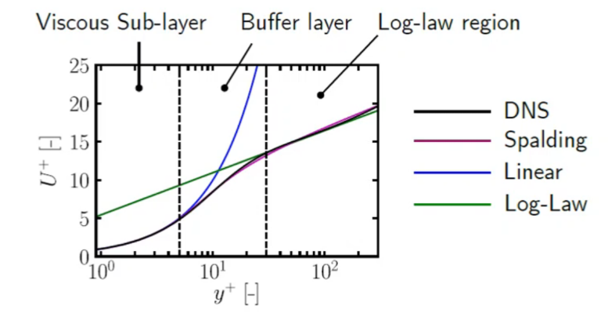
\includegraphics[width=0.7\linewidth]{02_Background/Figures/spalding_law-of-the-wall.png}
    \caption[Spalding law of the wall]{Dimensionless mean velocity profile in wall units: Spalding's law bridges the viscous sublayer, buffer layer and logarithmic region, approaching the linear and logarithmic limits. The DNS profile is shown for comparison. From \url{https://cfd.blogs.upv.es/turbulence/wall-functions/}[accessed December 2025]}
    \label{fig:background:spaldin_law-of-the-wall}
\end{figure}

\begin{figure}[H]
    \centering
    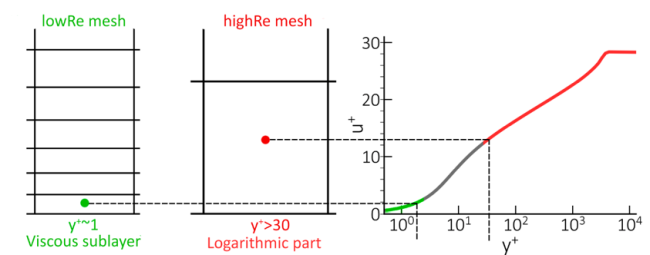
\includegraphics[width=\linewidth]{02_Background/Figures/wf_mesh.png}
    \caption[Wall-resolved and wall-function meshes]{Schematic comparison of a wall-resolved mesh (left), with its first cell centre in the viscous sublayer, and a conventional wall-function mesh (centre), with its first cell centre in the logarithmic region. The profile on the right indicates the corresponding locations in wall units. Reproduced from \url{https://ansyshelp.ansys.com/public/account/secured?returnurl=/Views/Secured/corp/v251/en/flu_th/section_kbf_dl4_vvb.html}[accessed September 2026]}
    \label{fig:background:wf-mesh}
\end{figure}

\subsection{Velocity transformations}
\label{subsec:background:velocity-transformations}
% Writing prerequisite for Chapter 7: distinguish a forward profile collapse
% from inversion of a transformation to recover wall shear at a matching point.
% State the property variations and inner-layer assumptions each law retains.

The freestream-normalized profiles in Figure~\ref{fig:background:dns-velocity-profiles} illustrate differences between the three cases, but do not directly test inner-layer similarity, which concerns \(u^+=u/u_\tau\). Compressible velocity transformations account for mean-property variations to relate the profiles to an approximately common law of the wall. Examples include the van Driest~\cite{van1951turbulent} and Trettel--Larsson~\cite{trettel2016mean} transformations, and the more recent formulations of Griffin et al.~\cite{griffin2021Transformation} and Hasan et al.~\cite{hasan2023incorporating}. Their accuracy and applicability depend on the flow conditions. The classical van Driest transformation retains \(y^+\), whereas the Trettel--Larsson and Griffin transformations use the semi-local coordinate \(y^*\). Figure~\ref{fig:background:trettel-larsson-profiles} illustrates the approximate collapse obtained with the Trettel--Larsson transformation. These transformations are not assessed individually here, the Griffin transformation is assessed indirectly through its role in the wall-function formulation~\cite{griffin2023WF}. Further discussion is given by Pecnik and Hasan~\cite{pecnik2026turbulence}.

\begin{figure}[H]
    \centering
    % Figure provenance:
    % Original vector export: tmp/boundary_layer_profile_comparison/trettel_larsson_velocity_ystar.pdf
    % Generating script: tmp/boundary_layer_profile_comparison/plot_trettel_larsson_ystar.py
    % Retained data: tmp/boundary_layer_profile_comparison/raw/
    % M6Tw076/M6Tw025: native zstar and Uvd_Trettel columns in *_Stat.dat;
    % Zhang, Duan and Choudhari (2018), DOI 10.2514/1.J057296.
    % C09: native y* and u* arrays (paper Eq. 20) from
    % https://www.klab.mech.tohoku.ac.jp/database/2025IwataniIJHFF/ustar-ystar-C09.txt
    % Iwatani, Asada and Kawai (2025), DOI 10.1016/j.ijheatfluidflow.2025.109896.
    % C09 station: Re_theta=1600, X=10.458614; differs from X=11 in earlier figures.
    % All coordinates and transformed velocities used unchanged; no C09 velocity factor.
    % Copied without cropping or resizing the source PDF.
    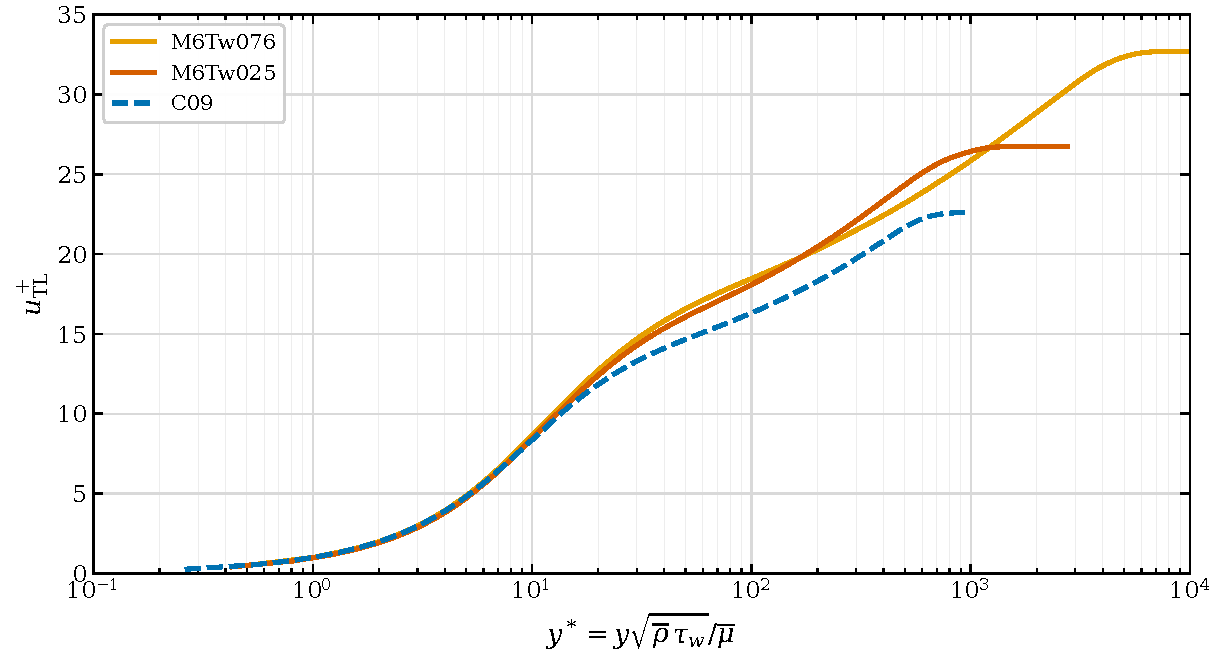
\includegraphics[width=\linewidth]{02_Background/Figures/trettel_larsson_velocity_ystar.pdf}
    \caption[Trettel--Larsson transformed DNS velocity profiles]{Trettel--Larsson transformed velocity \(u_{\mathrm{TL}}^+\) for M6Tw076 and M6Tw025~\cite{zhang2018direct} and the fully turbulent C09 case~\cite{iwatani2025subharmonic}, plotted against the semi-local coordinate \(y^*=y\sqrt{\overline{\rho}\tau_w}/\overline{\mu}\). In contrast to the freestream-normalized profiles in Figure~\ref{fig:background:dns-velocity-profiles}, the transformed profiles approximately collapse onto each other when both velocity and wall distance are transformed.}
    \label{fig:background:trettel-larsson-profiles}
\end{figure}

\subsection{Mean temperature-velocity relations - T(U)}
\label{subsec:background:temperature-velocity}
% Writing prerequisite for Chapter 7: present the mean T(U) or h(U) relations,
% their wall/reference states and cold-wall terms. Distinguish these mean
% relations (including GRA) from SRA statements about fluctuating quantities.
% Relate the wall slope to heat flux and explain the requirements for inversion.
The above mentioned velocity relation, serving as the momentum closure in wall-functions, needs a closure for the energy closure of the transport equations in the boundary layer is necessary. A similarity relation was found in the temperature-velocity relations - $T(U)$. Many of these relations exist, most notably by Crocco--Busemann, the Walz Relations \cite{walzcompressible}, by Duan-Martin \cite{duan2011direct_Part4}, or Zhang's Generalized Reynolds Analogy8 \cite{zhang2014generalized}. For a calorically perfect gas, the Crocco--Busemann and Walz relations, the Duan-Martin relation, and the mean temperature-velocity relation obtained from the generalized Reynolds analogy share a quadratic form (see Figure~\ref{fig:background:T-U-relation}). These analytical relations can be used in wall-functions to close the energy transport in the boundary layer. For the wall-function formulations investigated here, the mean \(T(U)\) relation supplies the thermal closure. Its accuracy is therefore an important additional criterion when assessing the RANS turbulence models coupled to these wall functions. It must be considered alongside \(U(y)\), \(T(y)\), their wall gradients and the resulting wall loads: agreement in \(T(U)\) alone does not establish the spatial temperature gradient, since \(\mathrm{d}T/\mathrm{d}y=(\mathrm{d}T/\mathrm{d}U)(\mathrm{d}U/\mathrm{d}y)\). Section~\ref{subsec:comparative:zpg:wr-profiles} applies these complementary assessments.

\begin{figure}[H]
    \centering
    % Figure provenance:
    % from publication: Zhang - A generalized Reynolds analogy for compressible wall-bounded turbulent flows
    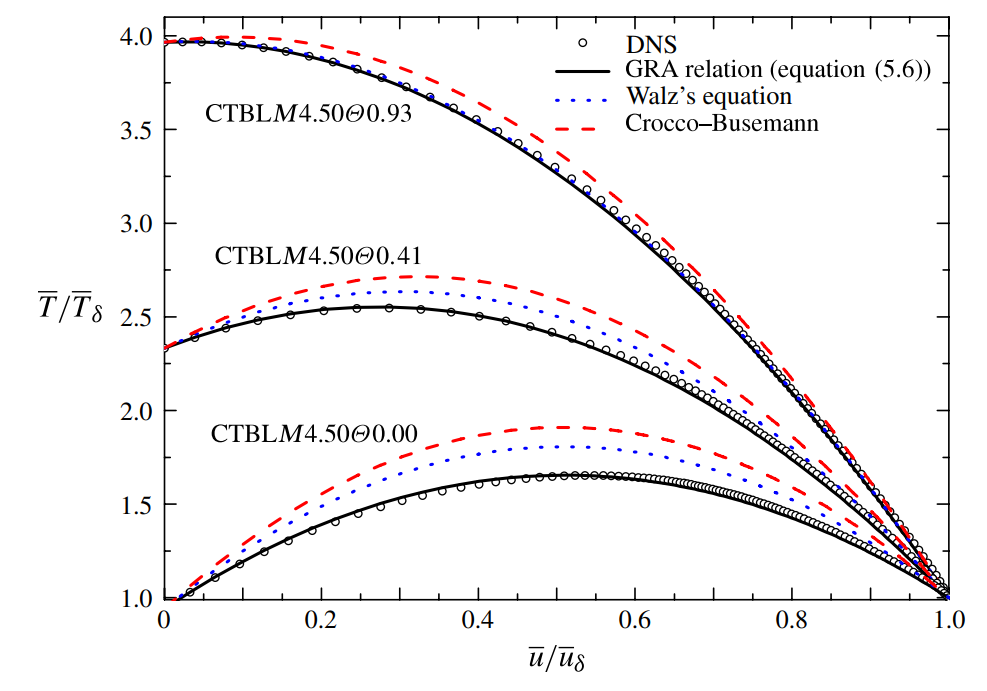
\includegraphics[width=0.85\linewidth]{02_Background/Figures/T-U-relations.png}
    \caption[introduction T(U) relations]{Mean \(T(U)\) relations for three Mach-4.5 turbulent flat-plate boundary layers with different wall thermal conditions, comparing the Crocco--Busemann, Walz and generalized Reynolds analogy relations with DNS. Reproduced from Zhang et al.~\cite{zhang2014generalized}.}
    \label{fig:background:T-U-relation}
\end{figure}


\subsection{Conclusion and implications to thesis work}

The possibility to describe the velocity and temperature boundary layer in universally similar fashion, allows for analytical descriptions of the boundary layer. With such analytical description the near-wall region need not be resolved anymore, but wall-functions based on these laws can be applied on coarse meshes. Conventional coarse wall-function meshes use a large wall-adjacent cell to span the modelled near-wall region (see Figure \ref{fig:background:wf-mesh}). The cold-wall profile shapes introduced in Section~\ref{sec:background:turbulent-boundary-layers-wall-heat-transfer} can make the associated internal-face spacing inadequate, as examined in Section~\ref{subsec:comparative:zpg:mesh-criterion}. Special formulations for the velocity and and temperature relations in hypersonic boundary layers are required, two wall-functions designed for these, by Li et al. \cite{li2025WF} and Griffin et al. \cite{griffin2023WF}, are being investigated in this thesis work (Section \ref{chap:wall-function-formulations}).